\section{Initial Results}
To assess long-term impacts of governor deadbands, thirty minutes of random load noise was applied to the miniWECC.
All governors had identical deadband settings and
PSLTDSim was used to set all governor droops to 5\%.
Some governors were removed from the system so that only $\approx$20\% of generation capacity in each area had governor control.
Each type of deadband shown in Fig. \ref{fig: deadbandType} was simulated.

Another experiment was conducted to explore a non-homogeneous deadband scenario where all deadbands were the same type, but some had different mHz deadbands.
Although PSLTDSim can model AGC, it was not enabled for any presented simulation.



\subsection{System Noise Injection}
At every time step, noise is injected into each load $P_{L,i}$ in the system according to
\begin{align}
P_{L,i} &= P_{L,i}(1 \pm N_Z Rand_i) \label{eq: noise}
\end{align}
where $N_Z$ represents the maximum amount of random noise to inject as a percent,
and $Rand_i$ is a randomly generated number between 0 and 1 inclusive.
The decision to add or subtract noise is chosen by another randomly generated number.
As described in \cite{AGCCresap}, (\ref{eq: noise}) creates random walk behavior in load that is representative of real power systems.


\subsection{Noise Simulation Results}

$N_Z$ was set to 0.03 for all simulations. 
The change in system loading caused by the noise is shown in Fig. \ref{fig: systemLoading}.
Fig. \ref{fig: sysFreqDB} shows the resulting system frequency for each type of deadband.
The step deadband holds frequency almost exactly on the set deadband except when system loading decreases during minutes 7-11.
The other deadband options maintain system frequency near their respective mHz setting until loading increases beyond a point near minute 17.
%After minute 17 the no-step and no deadband case frequency trend down faster than the non-linear deadband.


\begin{figure}[!ht]
\centering
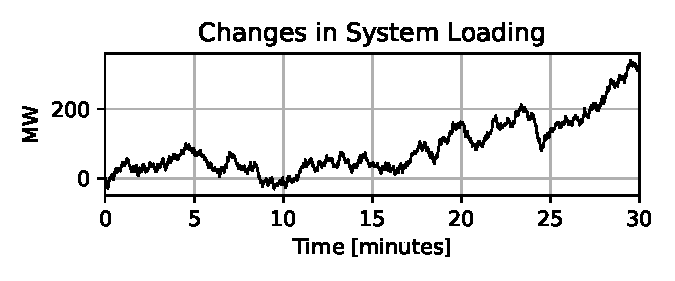
\includegraphics[width=\linewidth]{figures/miniWECCuniAccPloadChange}
\caption{Change in total system loading.}
\label{fig: systemLoading}
\end{figure}%
\begin{figure}[!ht]
\centering
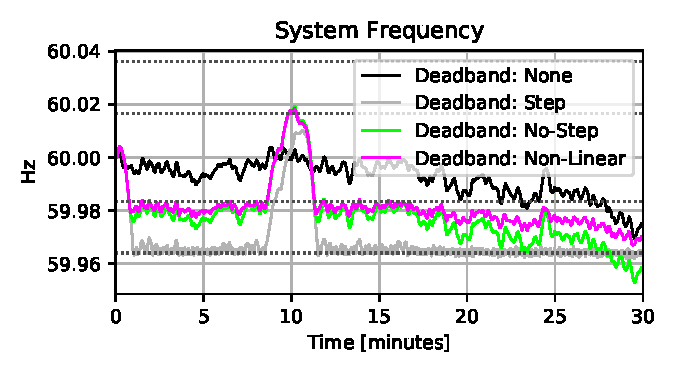
\includegraphics[width=\linewidth]{figures/miniWECCnoiseNLdroopDBFreq}
\caption{System frequency response of various deadband scenarios.}
\label{fig: sysFreqDB}
\end{figure}

Table \ref{tab: valveTravel} summarizes the valve travel for each generator in the system over the entire 30 minute simulation. 
A step type deadband has the largest total travel while the no-step deadband has the least.
%The no-step and no deadband cases have similar travel while the non-linear droop deadband has slightly more movement.

% Testing of external table build for \input later
% Uses the IEEE table format guidelines
\begin{table}[!ht]
	\caption{Total valve travel for various deadband scenarios.}
	\label{tab: valveTravel}
	\centering
	\begin{tabular}{@{} C{1cm} S[table-format=2.2] S[table-format=2.2] S[table-format=2.2] S[table-format=2.2] S[table-format=2.2] @{}} 	
							\toprule							
		&	\multicolumn{5}{c}{Valve Travel [PU]}							\\	
	\text{Generator}	&	\text{No DB}	&	\text{Step}	&	\text{No-Step}	&	\text{\shortstack{N-L\\Droop}}  &	\text{\shortstack{No-Step\\Non-H}}	\\	\midrule	
	17	&	0.16	&	7.48	&	0.15	&	0.23	& 0.19 \\	
	23	&	0.16	&	7.48	&	0.15	&	0.23	& 0.19 \\	
	30	&	0.16	&	7.48	&	0.15	&	0.23	& 0.19 \\	
	32	&	0.16	&	7.54	&	0.15	&	0.23	& 0.19 \\	
	107	&	0.16	&	7.54	&	0.15	&	0.23	& 0.19 \\	
	41	&	0.15	&	6.44	&	0.14	&	0.23	& 0.06 \\	
	45	&	0.15	&	6.44	&	0.14	&	0.23	& 0.06 \\	
	53	&	0.16	&	7.54	&	0.15	&	0.23	& 0.06 \\	
	59	&	0.15	&	6.44	&	0.14	&	0.23	& 0.06 \\	\bottomrule
	Total:	&	1.41	&	64.38	&	1.32	&	2.07& 1.19 	\\	

	\end{tabular}

\end{table}

The first three minutes of a single generators valve travel are shown in Fig. \ref{fig: valveComp} to compare how different deadbands affect valve movement.

\begin{figure}[!ht]
\centering
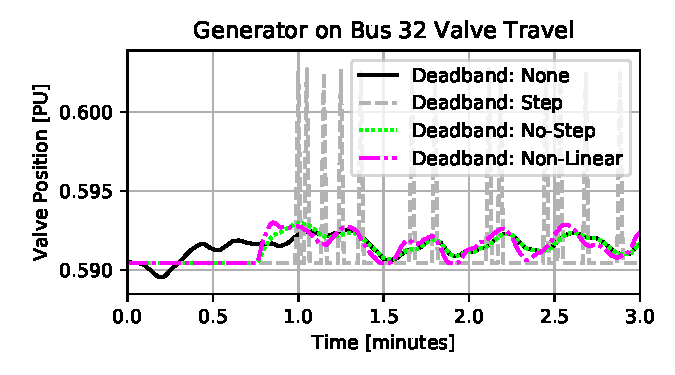
\includegraphics[width=\linewidth]{figures/gen32ValveComp}
\caption{Valve movement deadband comparisons.}
\label{fig: valveComp}
\end{figure}

A step deadband will send pulse train-esq control signals to the governor valve when system frequency is oscillating over the deadband. 
These repeated control pulses greatly increase valve travel over the more linear deadband options.
%The no-step deadband matches valve movement of the no deadband case after an initial delay.


\subsection{Non-Homogeneous Deadband Simulation Results}
With all governors using a no-step type deadband, two of the three areas mHz deadband was to 16.6 mHz while the third was set to 36 mHz.
The resulting system frequency is shown in Fig. \ref{fig: uniFreq}.
Individual valve travel for each generator is shown in {Table \ref{tab: valveTravel}} under the `No-Step Non-H' column, and Fig. \ref{fig: areaValveTravel} shows the average valve travel over time for each area.

\begin{figure}[!ht]
\centering
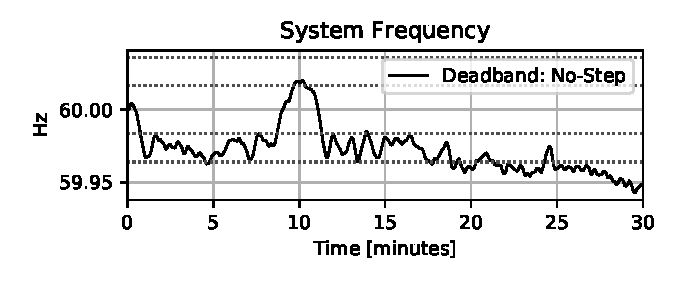
\includegraphics[width=\linewidth]{figures/miniWECCuniAccFreq}
\caption{System frequency response to 0.03\% load noise where no-step deadbands have different settings.}
\label{fig: uniFreq}
\end{figure}

\begin{figure}[!ht]
\centering
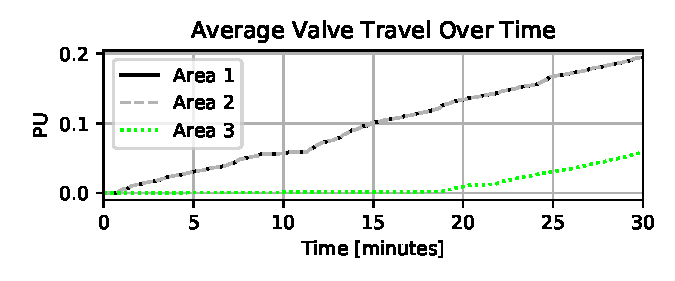
\includegraphics[width=\linewidth]{figures/miniWECCuniAccVTOverTime}
\caption{Average valve travel by area for non-homogeneous deadband test.}
\label{fig: areaValveTravel}
\end{figure}

As expected, governors with a larger deadband won't respond until after frequency drops below their deadband while governors with smaller deadbands work to maintain frequency. 
In this case, the governor valves with a smaller deadband move three times more than those with a larger deadband even though total system valve movement is reduced from the homogeneous no-step scenario.

